\documentclass[10pt,a4paper]{ctexart}
\usepackage[utf8]{inputenc}
\usepackage{amsmath}
\usepackage{amsfonts}
\usepackage{amssymb}
\usepackage{graphicx}
\usepackage{xcolor}
\usepackage{bm}
\author{吴秉哲}
\title{数值分析上机报告}
\begin{document}
\maketitle
这学期每次的上机报告都按如下格式编写:

每份报告分为几个章节,每个章节分别介绍上机作业中的一题,其中每个
题目又分为以下几个部分:
\begin{enumerate}
\item 问题提出及相关背景知识
\item 问题的理论分析及解决方案
\item 程序的部分设计思路与细节
\item 计算成果与分析
\item 本次上机的反思
\end{enumerate}
每个题目中要求回答的问题均蕴含在问题的理论分析与计算成果分析两部分

在程序方面,都是由C++编写完成(其中用到了自己编写的库:矩阵(Matrix),向量(Vector),以及数值代数的相关算法(linear)),在linux下由g++编译。数据方面
一般使用matlab可视化处理,少部分使用了python。

\section{第五章第一题}
\subsection{问题提出及相关背景知识}
题目给出一个严格对家占优的循环矩阵,要求对$N=2^{10}$用FFT的方法解对应的方程组,并与共轭梯度法比较。
\subsection{问题的理论分析及解决方案}
由于所解方程的系数矩阵为严格对家占优的循环矩阵,则可以推导出其为正定对称矩阵,进而可以使用PCG(预优共轭梯度法)进行数值求解。
又由于其为循环矩阵,由教材的推导,可以使用离散傅立叶变化求解,当矩阵的阶数$N=2^n$时,还可以使用FFT加速。

在本题的上机中,直接选取对角矩阵为预优矩阵。
\subsection{程序设计的思路与细节}
本次上机程序设计的主要难点为FFT算法的实现,我在程序中使用了递归来实现FFT。值得一提FFT的算法可以有两种思路,一种为教材的思路,
还有一种从信号处理的角度来看,可以对所变化向量从频域上划分,也可以作类似的实现。我在我的程序Fourier.h中,对这两种方法都有实现。
\subsection{计算成果与分析}
首先给出题目要求的几个特殊结果,然后列出进一步实验的一些数据,最后对两种方法进行分析。

取$N=2^{10}$时,用FFT解对应方程组所得到的结果达到了机器精度,花费了0.006s。取$N=100,N=150$时,PCG法均在迭代8步以内得到了机器精度
的解。

下面我们看一看进一步的结果。

不难看出所求方程组的精确解为$(0.5,0.5,\cdots,0.5)^T$,而进行实验方法都可以在一定条件下达到机器精度,于是我主要通过控制相同精度,然后

取$2^{n},n=1,2,\cdots,10$为系数矩阵的阶数,观察两种方法所需要的时间,并将其做可视化处理得到了下面一张图表:
\par
\centerline{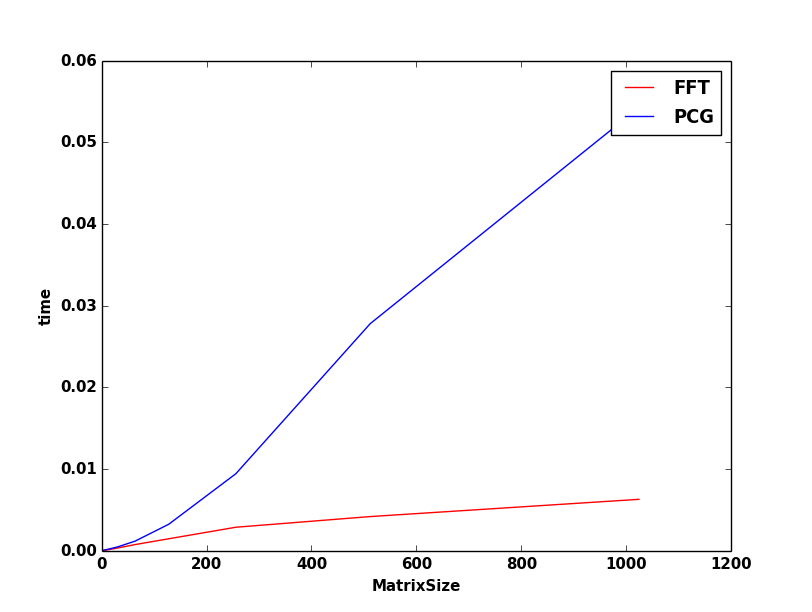
\includegraphics[height=7cm,width=10cm]{fft1.png}}
\par
在上图中,红线表示FFT方法随着N的变化所需时间的变化,而蓝线表示PCG法。
从上图明显可以看出FFT与PCG法所花费时间的差异,共轭梯度法的时间负责度为$O(N^2)$,而FFT为$O(Nlog(N))$,图像与之相符合。
\subsection{本次上机反思}
在这个题的充分感受到了FFT在解某些特殊问题的优势,以后在解决类似问题的时候,如果问题的规模较大,可以优先考虑使用
离散傅立叶变化来解决,进而可以用FFT进行加速。
\section{第五章第二题}
\subsection{问题提出及相关背景知识}
题目给出了两个非周期的具有紧支集的向量,要求计算非周期的卷积。具有紧支集可以得到该向量的分量只有有限个不为0。本题
具有信号处理的学科背景,具体见下一节的分析。
\subsection{问题的理论分析及解决方案}
本题来源于信号处理,信号处理中经常需要求两个离散信号的卷积,但是一般求周期卷积的方法比较简单,信号处理中周期卷积也叫循环卷积。但是我们
在实际问题中常常遇到题目中的这种普通卷积,这时根据信号处理中的循环卷积定理可以将普通卷积的计算转化为循环卷积的计算。

由于本题所给的卷积为两个向量的非周期卷积(教材所给方法为计算循环卷积的情形),所以需要对教材FFT求循环卷积的方法进行一定的修改,具体做法如下:

记$N_0=M+Q-1$,选取大小适当的$n$满足$N=2^n\geq N$,比如在本题条件$Q=200,M=500$时,可以取$N=1024$,这时就可以根据教材的方法计算
$(x_1,x_2,\cdots,x_N)$与$(h_1,h_2,\cdots,h_N)$的周期卷积,然后根据周期卷积定理,所求的的卷积即为题目所求的非周期的卷积的前N个分量,
其余分量为0。

综上,就求得所要求的非周期卷积。
\subsection{计算结果分析}

由上面的推导,在计算推导中出现的周期卷积的时候既可以用FFT来做,也可以使用卷积的定义(教材这里不够严谨,教材给的是循环卷积的定义,应该与一般的卷积区分)。下面先列出计算结果的图($x_n,h_n,(x*h)_n$)的离散图像:
\par
\centerline{\includegraphics[height=5cm,width=12cm]{5.2.png}}
\par
\par
\centerline{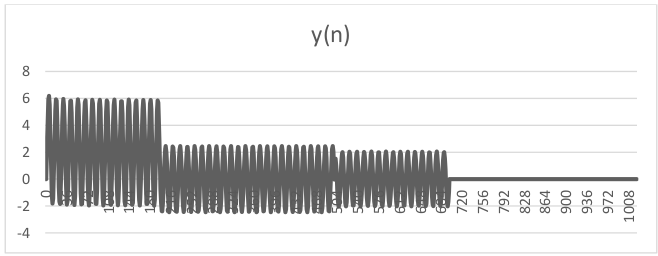
\includegraphics[height=5cm,width=12cm]{5.21.png}}
\par
从上图可以看出最后得到的卷积的图像的特点是信号的能量不停衰减最后到0,这也可以通过对两个信号进行理论上的分析得到。还有一点要提一下的是在电脑上
上机实现FFT变化时涉及到复数运算,我用的是C++ STL模板中的complex模板,这样由于舍入误差的存在,实向量做FFT后最后得到的结果的虚部一般会是一个很小的数,我一般直接舍弃。

下面,我实验了不同大小的$M,Q$,然后比较两种方法在时间上的差异,最后如上题一样绘制了图像,结果如下:
\par
\centerline{\includegraphics[height=7cm,width=10cm]{../vim/5.2.png}}
\par
从上面可以看出FFT方法在花费时间上巨大的优势。
\section{第五章第三题}
\subsection{问题提出及相关背景知识}
这个问题还是来源与信号处理中消除白噪声问题。原题给出一个信号$f(t)$,题目要求做这样的处理:将原信号做离散傅立叶变化后,去掉其中的
高频项,然后做傅立叶反变化,得到一个新信号。题目要求对比原信号图像与新得到的信号的图像的差别。
\subsection{问题理论分析及相关背景知识}
这个问题程序实现起来比较容易。主要要理解它背后的思想,即从消除信号的噪声的角度,来理解离散傅立叶变换在其中起到的作用。

首先我们将输入信号做频谱变化(即第一次FFT),去掉其中的噪声,由信号处理方面的知识,噪声即为做变换后的高频部分,所以过滤掉高频
部分就可以达到消除噪声的效果,而教材题目给的方法为给定m,令高频部分为0,这其实就是信号处理中截断函数的另一种提法下面我们来看看这种方法的实际效果。
\subsection{计算结果分析}
首先我们用Python画出原始信号的图像,如下:
\par
\centerline{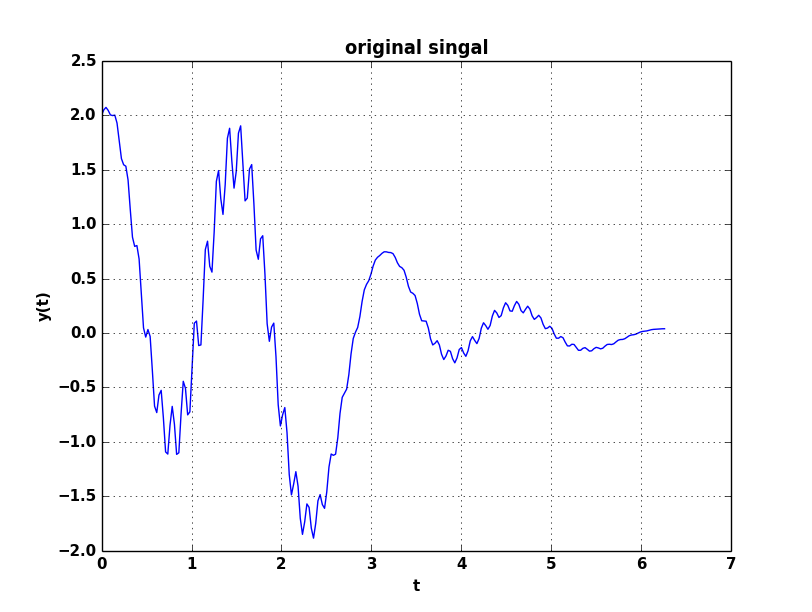
\includegraphics[height=7cm,width=12cm]{singal0.png}}
\par
从上图可以看出,信号受噪声的影响还是很明显的。下面我们来看看处理过后的信号的图像(图像为题目中$m=6$时):
\par
\centerline{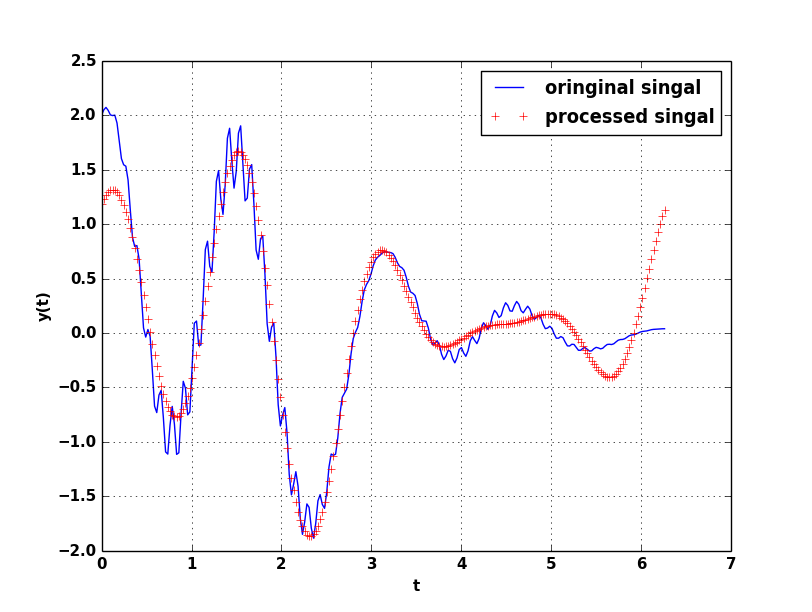
\includegraphics[height=7cm,width=12cm]{singal1.png}}
\par
由对比图可以发现此种方法消除噪声的效果特别明显.

进一步实验,改变m的值,可以发现当m越大时,所得的信号与原始信号越接近,也就是消除噪声的效果减弱了,由于篇幅原因,就不再画图对比了。

以上就是整个信号消噪的过程,在以后实际应用中,还可能需要构造不同的截断函数对信号处理,这就不属于数值分析的范畴了。
\end{document}
